\scanpage{57}
\deleted{est déterminée par la structure de graphe avec un sommet particulier \unsure{par le}}

Les cas les plus simples sont les cas élémentaires (graphes \deleted{à un \unsure{pt}} \inserted{ponctuels})
\margin{MD-graphes élémentaires (sommet isolé \inserted{\unsure{i.e. de dim modulaire nulle|i.e. en dim modulaire nulle}}) de dim. modulaire $1$ \deleted{\illegible{1}} \deleted{\unsure{de dim}\ $1$}}
\figure{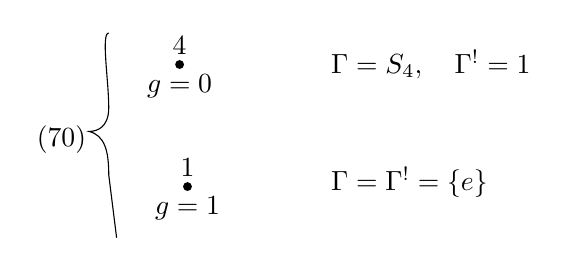
\begin{tikzpicture}[x=1cm,y=1cm]
\node at (-1.3,-.75) {$(70)$};\draw (-.7,.6) .. controls (-.8,.6) and (-.7,0) .. (-.7,-.35) .. controls (-.7,-.6) and (-.85,-.65) .. (-.95,-.65) .. controls (-.75,-.7) and (-.7,-.9) .. (-.7,-1.2) -- (-.6,-2);
\fill (.2,.2) circle(1.6pt);\node[above] at (.2,.2) {$4$};\node[below] at (.2,.2) {$g=0$};\node[right] at (2,.2) {$\Gamma=\unsure{\mathfrak S}_4,\quad\Gamma^!=1$};
\fill (.3,-1.35) circle(1.6pt);\node[above] at (.3,-1.35) {$1$};\node[below] at (.3,-1.35) {$g=1$};\node[right] at (2,-1.3) {$\Gamma=\Gamma^!=\{e\}$};
\end{tikzpicture}}
Les autres cas sont ceux des \inserted{MD-}graphes ``\uline{rationnels}'' (tous les $g_\alpha$ nuls) tels que tous les $\widehat\nu_\alpha$ soient égaux à trois (donc les sommets d'ordre $1\leq\widetilde\mu_\alpha\leq3$) \deleted{\unsure{et un}} \inserted{sauf l'}un d'eux, qui est égal à $4$ (donc $1\leq\widetilde\mu_{\alpha_0}\leq4$), ou bien des \inserted{MD-}graphes qui ont tous leurs sommets sauf un rationnels et $\widehat\nu_\alpha=3$, \deleted{(donc} sauf un \inserted{$\alpha_0$} qui est un sommet-bout ($\widetilde\mu_\alpha=1$) et de genre $1$, $\nu_{\alpha_0}=0$ --- donc ici tous les sommets sont d'ordre $1\leq\widetilde\mu_\alpha\leq3$, et les $\nu_\alpha$ \inserted{pour $\alpha\ne\alpha_0$} sont égaux à $3-\widetilde\mu_\alpha$, \deleted{pour $\alpha\ne$} et $\nu_{\alpha_0}=0$.

Dans l'un et l'autre cas \inserted{($g_{\alpha_0}=0$, $g_{\alpha_0}=1$)} on aura un iso can. de multiplicités
\[
\text{(71)}\qquad\widehat M_G\simeq\widehat M_{g_{\alpha_0},\widehat I_{\alpha_0}}
\]
\margin{avec $\widehat I_{\alpha_0}=I_{\alpha_0}+\widetilde A_{\alpha_0}$ (de cardinal $4$ ou $1$ suivant que $g_{\alpha_0}=0$ ou $g_{\alpha_0}=1$)}
\margin{56}
